\documentclass[11pt,a4paper]{article}

\usepackage[margin=1in]{geometry}
\usepackage{amsmath,amssymb}
\usepackage{booktabs}
\usepackage{graphicx}
\usepackage{hyperref}
\usepackage{caption}
\usepackage{subcaption}
\usepackage{enumitem}

\hypersetup{
  colorlinks=true,
  linkcolor=blue,
  urlcolor=blue,
  citecolor=blue
}

\graphicspath{{outputs/}}

\title{Exploration--Exploitation Algorithms for Credit Scoring}
\author{Samrawit Kahsay\\Student ID: UGR/2271/14}
\date{\today}

\begin{document}
\maketitle

\begin{abstract}
We study three multi-armed bandit algorithms---$\varepsilon$-greedy, Upper Confidence Bound (UCB1), and Thompson Sampling for Bernoulli rewards---in a credit scoring context where each arm is a repeat-borrower segment and rewards encode repayment success. Over $T{=}5000$ borrower interactions and $50$ Monte Carlo simulations, UCB1 with exploration coefficient $c{=}0.25$ achieved the highest mean total reward ($3634.3$ successful repayments), while Thompson Sampling converged fastest ($t^\ast{=}6$) and concentrated most strongly on the true best segment in the final $10\%$ of pulls (tail best-arm rate $0.84$). We compare exploration efficiency, exploitation effectiveness, convergence, and suitability for adaptive credit scoring using cumulative reward, average reward, and arm-selection frequency plots.
\end{abstract}

\section{Introduction}

Credit institutions increasingly score \emph{repeat borrowers} using past repayment behavior. When several borrower segments, policy tiers, or applicant categories are available, the lender must balance \textbf{exploration} (trying less-understood groups to learn their repayment rates) and \textbf{exploitation} (allocating decisions to groups believed most creditworthy). This assignment frames that problem as a \textbf{multi-armed bandit}: each arm is a segment; each interaction yields a Bernoulli reward ($1$ = repayment, $0$ = default).

We implement and evaluate:
\begin{enumerate}[noitemsep]
  \item $\varepsilon$-greedy exploration,
  \item UCB1 with tunable exploration parameter $c$,
  \item Thompson Sampling with Beta--Bernoulli posteriors.
\end{enumerate}

\section{Problem Setup}

\subsection{Arms and rewards}

We simulate $K{=}6$ repeat-borrower segments with true repayment probabilities
\[
\mathbf{p} = (0.58,\; 0.61,\; 0.65,\; 0.69,\; 0.72,\; 0.74).
\]
Arm $5$ is the most creditworthy ($p^\ast = 0.74$). At each step $t \in \{1,\ldots,T\}$, an algorithm selects an arm $a_t$, observes $r_t \sim \mathrm{Bernoulli}(p_{a_t})$, and updates estimates used as \textbf{creditworthiness scores} for ranking segments.

\subsection{Metrics}

Over $S{=}50$ independent simulations we report:
\begin{itemize}[noitemsep]
  \item \textbf{Mean total reward}: $\bar{R} = \frac{1}{S}\sum_s \sum_{t=1}^T r_t^{(s)}$.
  \item \textbf{Mean average reward}: $\bar{R}/T$.
  \item \textbf{Mean regret}: $T p^\ast - \bar{R}$ (oracle always pulls the best arm).
  \item \textbf{Tail best-arm rate}: fraction of pulls of arm $5$ in the last $10\%$ of steps.
  \item \textbf{Convergence $t^\ast$}: first step where running average reward $\geq 0.95\, p^\ast$ (lower is faster).
  \item \textbf{Mean final ranking}: arms ordered by learned value estimates (descending).
\end{itemize}

Experiments use $T{=}5000$, $S{=}50$, seed $7$ (see \texttt{run\_experiments.py}).

\section{Algorithms}

\subsection{Epsilon-greedy}

With probability $\varepsilon$, select a uniform random arm; otherwise exploit the arm with highest sample-mean reward $\hat{\mu}_a$. Incremental updates: $\hat{\mu}_a \leftarrow \hat{\mu}_a + (r - \hat{\mu}_a)/n_a$.

\subsection{UCB1}

After an initial pull of each arm, select
\[
a_t = \arg\max_a \left( \hat{\mu}_a + c \sqrt{\frac{2 \ln t}{n_a}} \right),
\]
where $c \geq 0$ controls optimism toward under-sampled arms.

\subsection{Thompson Sampling (Bernoulli)}

Maintain $\mathrm{Beta}(\alpha_a, \beta_a)$ posteriors per arm. Each step sample $\tilde{\theta}_a \sim \mathrm{Beta}(\alpha_a,\beta_a)$, play $\arg\max_a \tilde{\theta}_a$, then update $\alpha_a \mathrel{+}= r$, $\beta_a \mathrel{+}= 1-r$.

\section{Experimental Results}

\subsection{Epsilon-greedy sweep}

Table~\ref{tab:epsilon} summarizes the effect of $\varepsilon$ on exploration versus exploitation.

\begin{table}[htbp]
  \centering
  \caption{Epsilon-greedy sweep ($T{=}5000$, $S{=}50$).}
  \label{tab:epsilon}
  \begin{tabular}{lrrrrr}
    \toprule
    Setting & Total reward & Avg reward & Regret & Tail best-arm & $t^\ast$ \\
    \midrule
    $\varepsilon = 0.01$ & 3575.7 & 0.7151 & 124.3 & 0.555 & 268 \\
    $\varepsilon = 0.05$ & \textbf{3622.7} & \textbf{0.7245} & \textbf{77.3} & \textbf{0.708} & 96 \\
    $\varepsilon = 0.10$ & 3614.1 & 0.7228 & 85.9 & 0.690 & 239 \\
    $\varepsilon = 0.20$ & 3587.0 & 0.7174 & 113.0 & 0.640 & 91 \\
    \bottomrule
  \end{tabular}
\end{table}

\textbf{Observation.} $\varepsilon{=}0.05$ dominates the sweep: $47.0$ more successful repayments than $\varepsilon{=}0.01$ and $35.7$ more than $\varepsilon{=}0.20$, with the lowest regret ($77.3$). Very small $\varepsilon{=}0.01$ under-explores (regret $124.3$, slow $t^\ast{=}268$). Larger $\varepsilon$ values waste pulls on random segments after the best arm is identifiable, lowering total reward.

\begin{figure}[htbp]
  \centering
  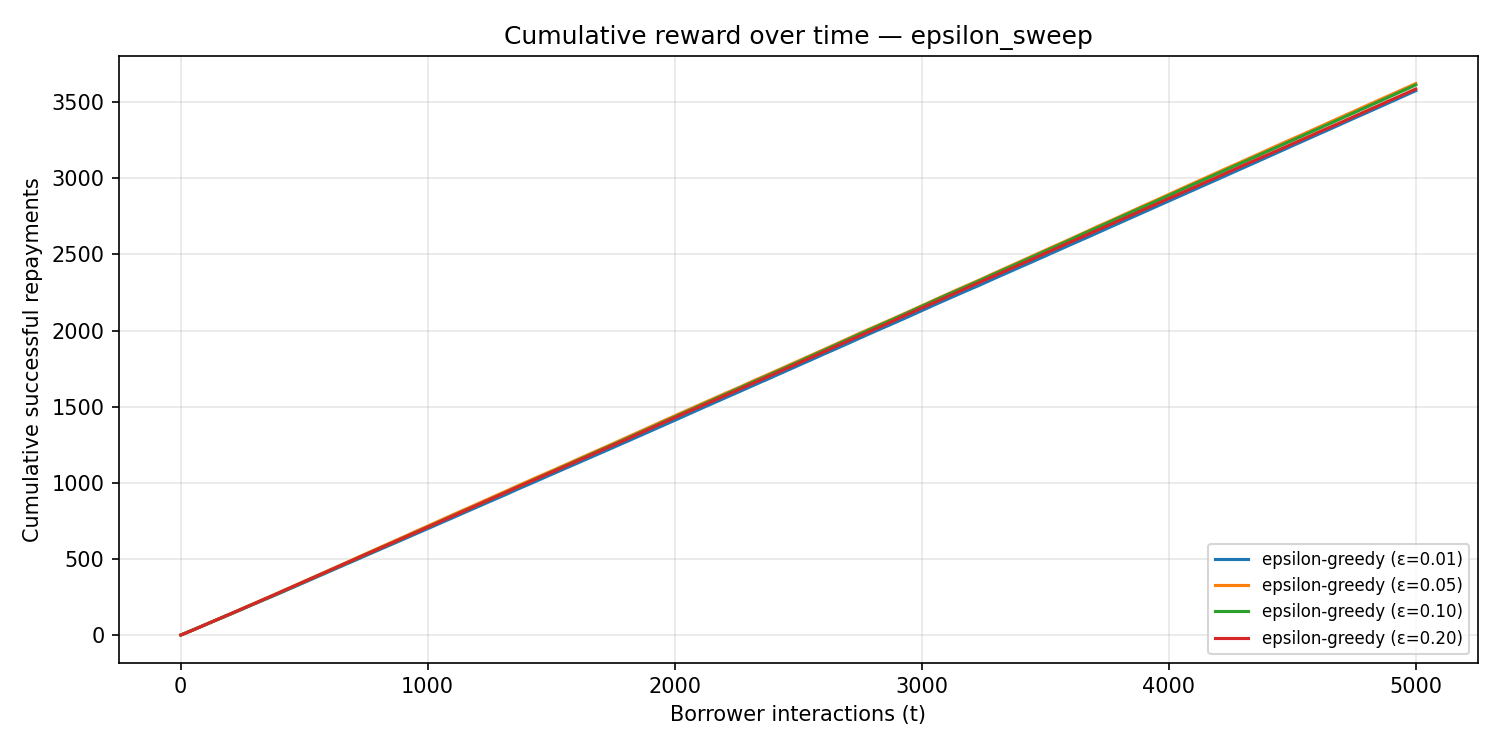
\includegraphics[width=0.95\linewidth]{epsilon_sweep__cumulative_reward.png}
  \caption{Cumulative reward over time---epsilon-greedy sweep.}
  \label{fig:eps-cum}
\end{figure}

\begin{figure}[htbp]
  \centering
  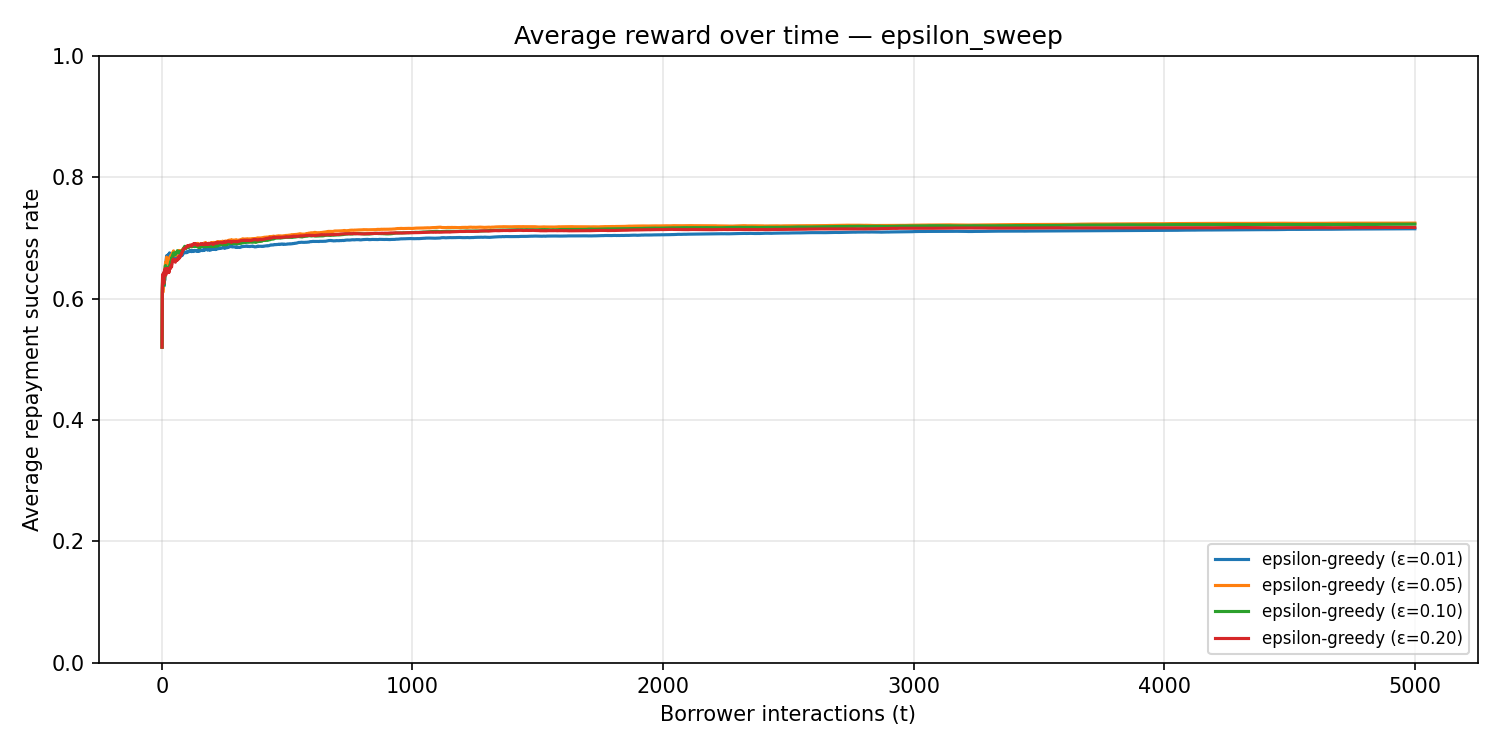
\includegraphics[width=0.95\linewidth]{epsilon_sweep__average_reward.png}
  \caption{Average repayment success rate over time---epsilon-greedy sweep.}
  \label{fig:eps-avg}
\end{figure}

\begin{figure}[htbp]
  \centering
  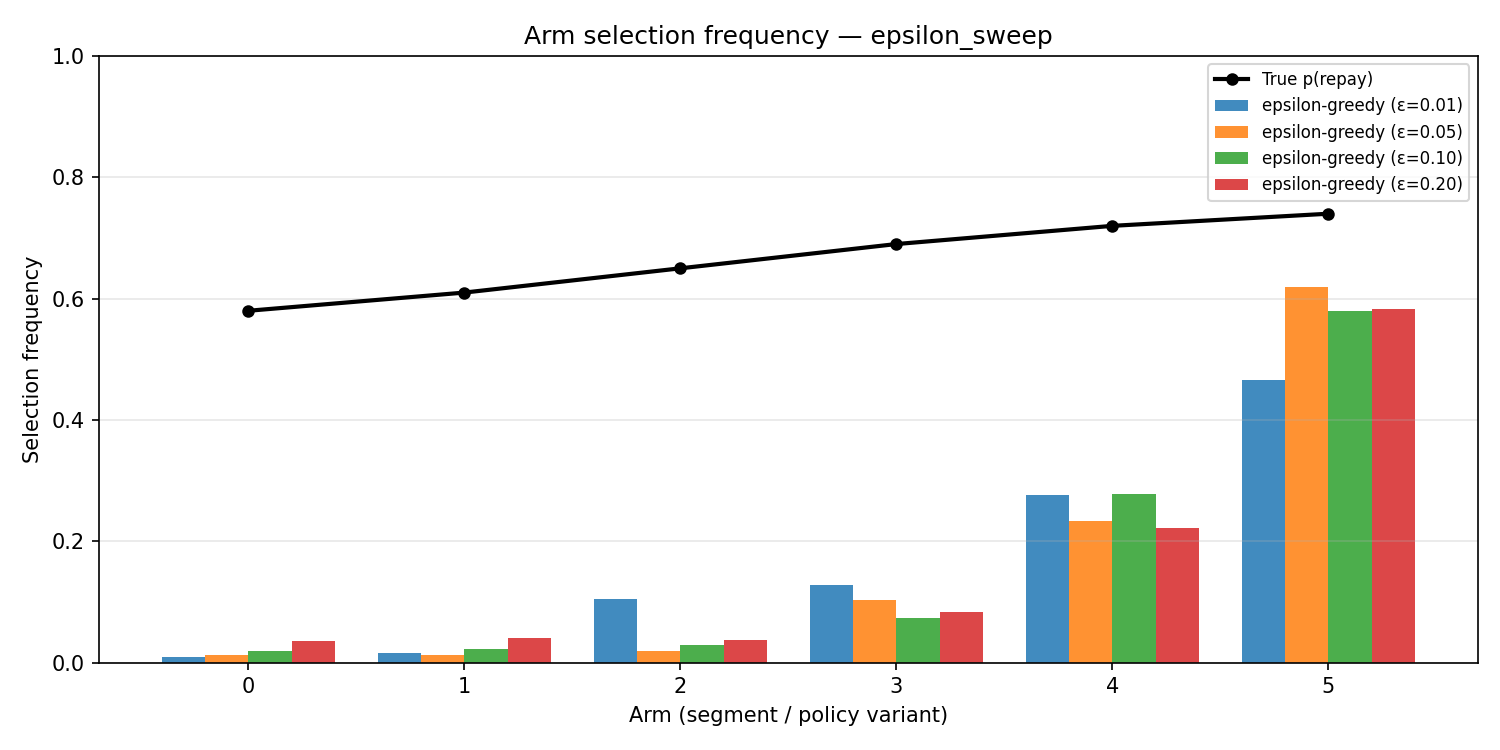
\includegraphics[width=0.85\linewidth]{epsilon_sweep__arm_frequencies.png}
  \caption{Arm selection frequencies vs.\ true repayment probabilities---epsilon-greedy sweep.}
  \label{fig:eps-freq}
\end{figure}

\subsection{UCB sweep}

Table~\ref{tab:ucb} shows how the exploration coefficient $c$ affects performance.

\begin{table}[htbp]
  \centering
  \caption{UCB1 sweep ($T{=}5000$, $S{=}50$).}
  \label{tab:ucb}
  \begin{tabular}{lrrrrr}
    \toprule
    Setting & Total reward & Avg reward & Regret & Tail best-arm & $t^\ast$ \\
    \midrule
    $c = 0.25$ & \textbf{3634.3} & \textbf{0.7269} & \textbf{65.7} & \textbf{0.718} & 16 \\
    $c = 0.50$ & 3594.9 & 0.7190 & 105.1 & 0.694 & 51 \\
    $c = 1.00$ & 3503.5 & 0.7007 & 196.5 & 0.451 & 182 \\
    $c = 2.00$ & 3429.0 & 0.6858 & 271.0 & 0.300 & 23 \\
    \bottomrule
  \end{tabular}
\end{table}

\textbf{Observation.} Smaller $c{=}0.25$ yields the best total reward and lowest regret. As $c$ increases, UCB over-explores: total reward drops by $205.3$ from $c{=}0.25$ to $c{=}2.00$, and tail best-arm rate falls from $0.718$ to $0.300$, indicating weaker late-stage focus on arm~5.

\begin{figure}[htbp]
  \centering
  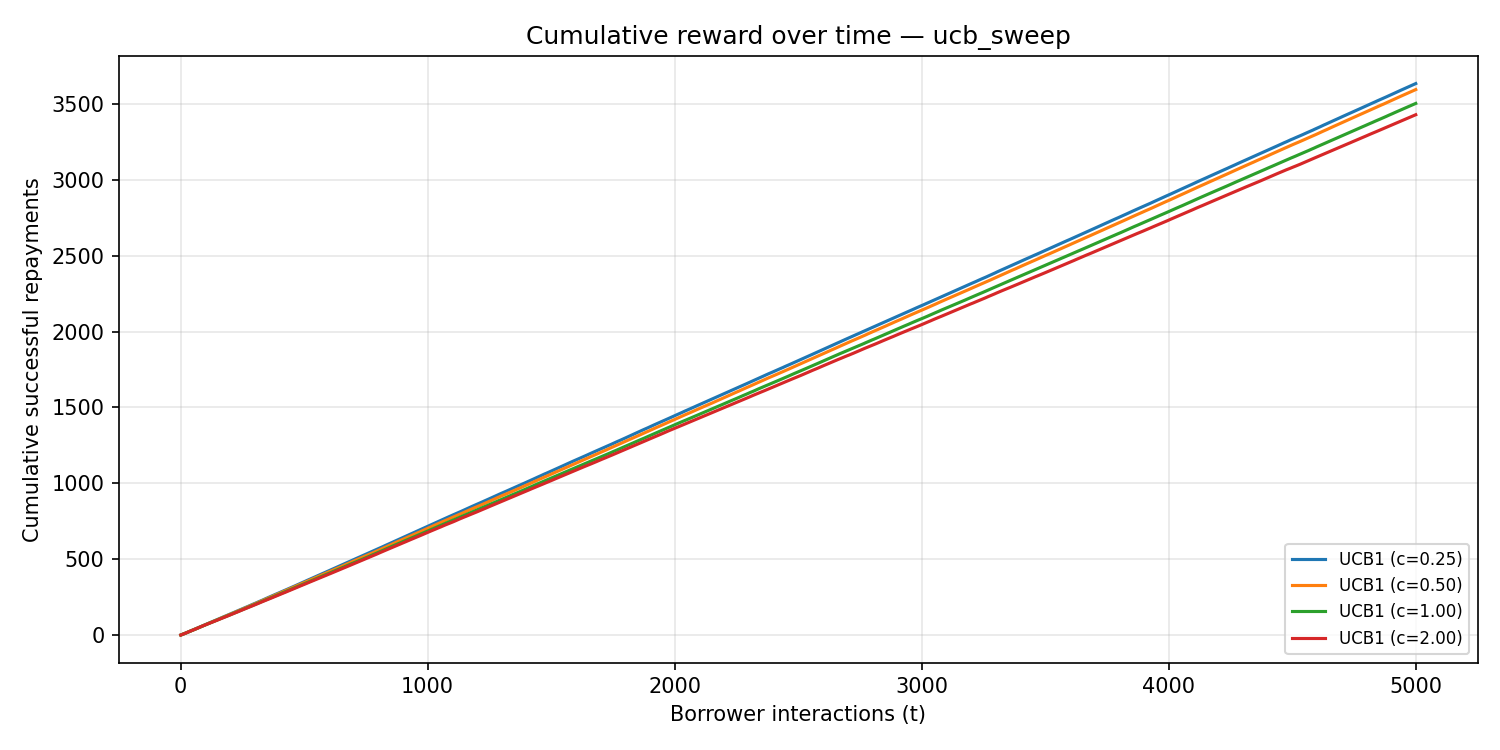
\includegraphics[width=0.95\linewidth]{ucb_sweep__cumulative_reward.png}
  \caption{Cumulative reward over time---UCB sweep.}
  \label{fig:ucb-cum}
\end{figure}

\begin{figure}[htbp]
  \centering
  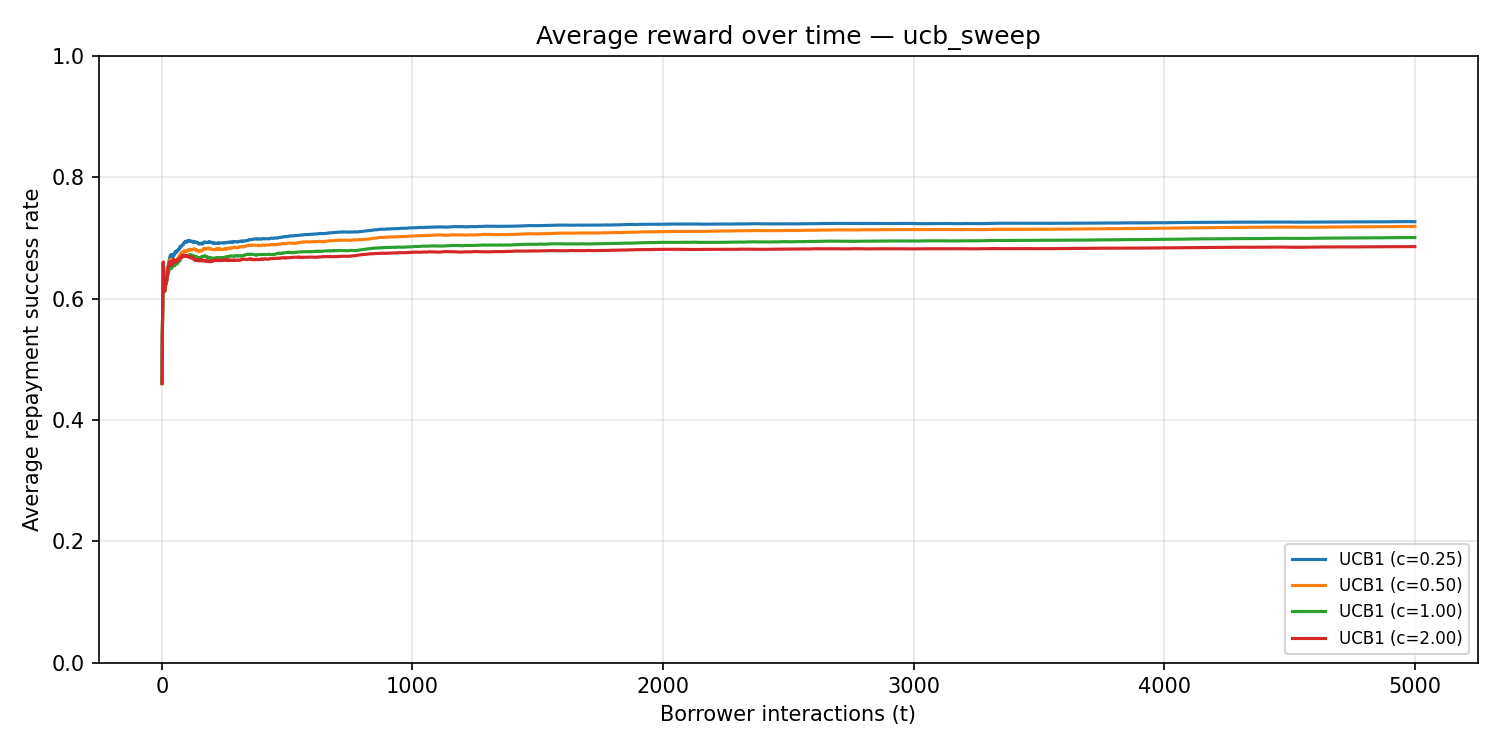
\includegraphics[width=0.95\linewidth]{ucb_sweep__average_reward.png}
  \caption{Average repayment success rate over time---UCB sweep.}
  \label{fig:ucb-avg}
\end{figure}

\begin{figure}[htbp]
  \centering
  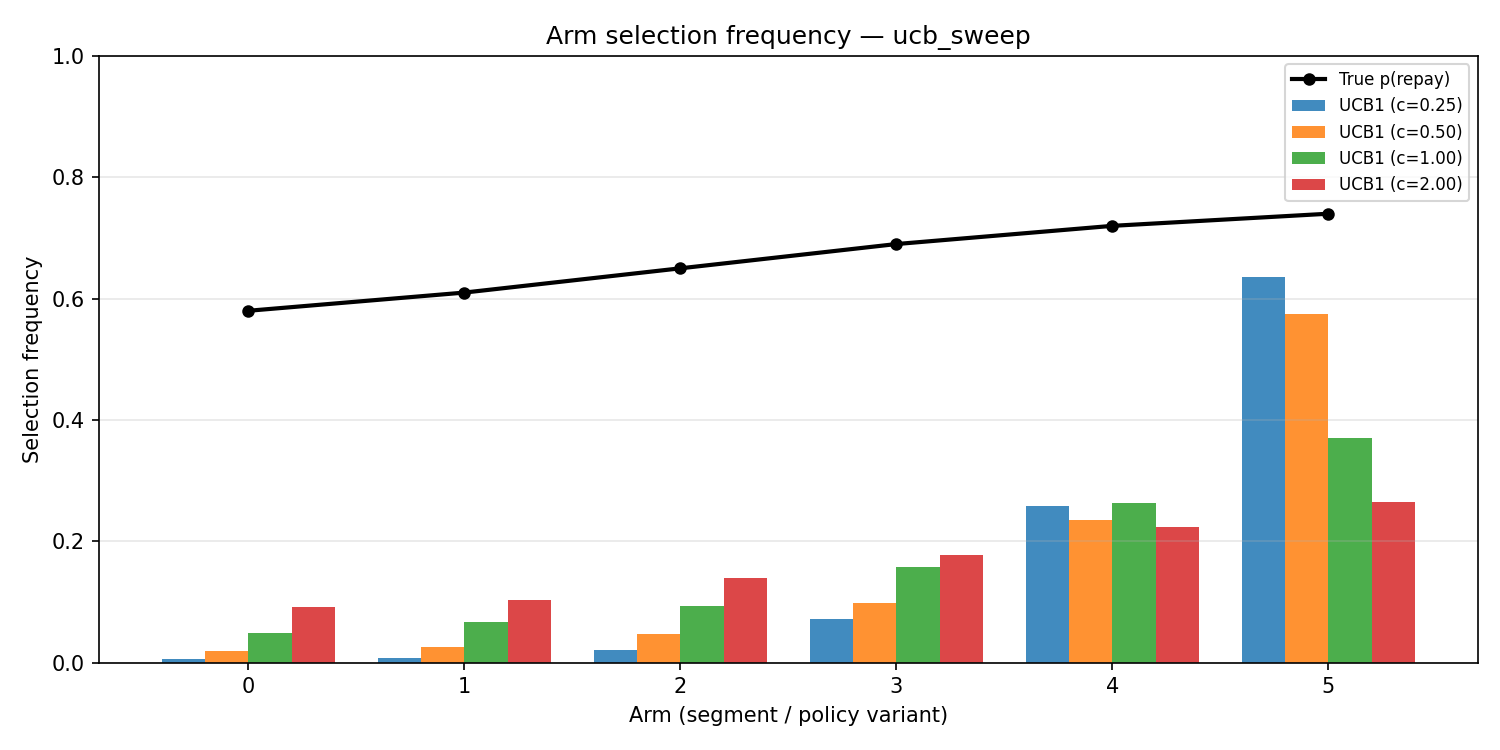
\includegraphics[width=0.85\linewidth]{ucb_sweep__arm_frequencies.png}
  \caption{Arm selection frequencies---UCB sweep.}
  \label{fig:ucb-freq}
\end{figure}

\subsection{Final comparison}

Table~\ref{tab:comparison} compares the best hyperparameters from each sweep against Thompson Sampling.

\begin{table}[htbp]
  \centering
  \caption{Final comparison: best $\varepsilon$-greedy, best UCB1, Thompson Sampling.}
  \label{tab:comparison}
  \begin{tabular}{lrrrrrl}
    \toprule
    Method & Total reward & Avg reward & Regret & Tail best-arm & $t^\ast$ & Ranking \\
    \midrule
    $\varepsilon$-greedy ($\varepsilon{=}0.05$) & 3622.7 & 0.7245 & 77.3 & 0.708 & 96 & $5{>}4{>}3{>}2{>}1{>}0$ \\
    UCB1 ($c{=}0.25$) & \textbf{3634.3} & \textbf{0.7269} & \textbf{65.7} & 0.718 & 16 & $5{>}4{>}3{>}2{>}1{>}0$ \\
    Thompson Sampling & 3626.4 & 0.7253 & 73.6 & \textbf{0.840} & \textbf{6} & $5{>}4{>}3{>}2{>}1{>}0$ \\
    \bottomrule
  \end{tabular}
\end{table}

The oracle benchmark is $T p^\ast = 5000 \times 0.74 = 3700$ repayments. UCB1 ($c{=}0.25$) comes closest ($65.7$ regret). Thompson Sampling ranks second on total reward ($3626.4$) but achieves the fastest convergence ($t^\ast{=}6$) and the strongest late exploitation of the best arm (tail rate $0.84$).

\begin{figure}[htbp]
  \centering
  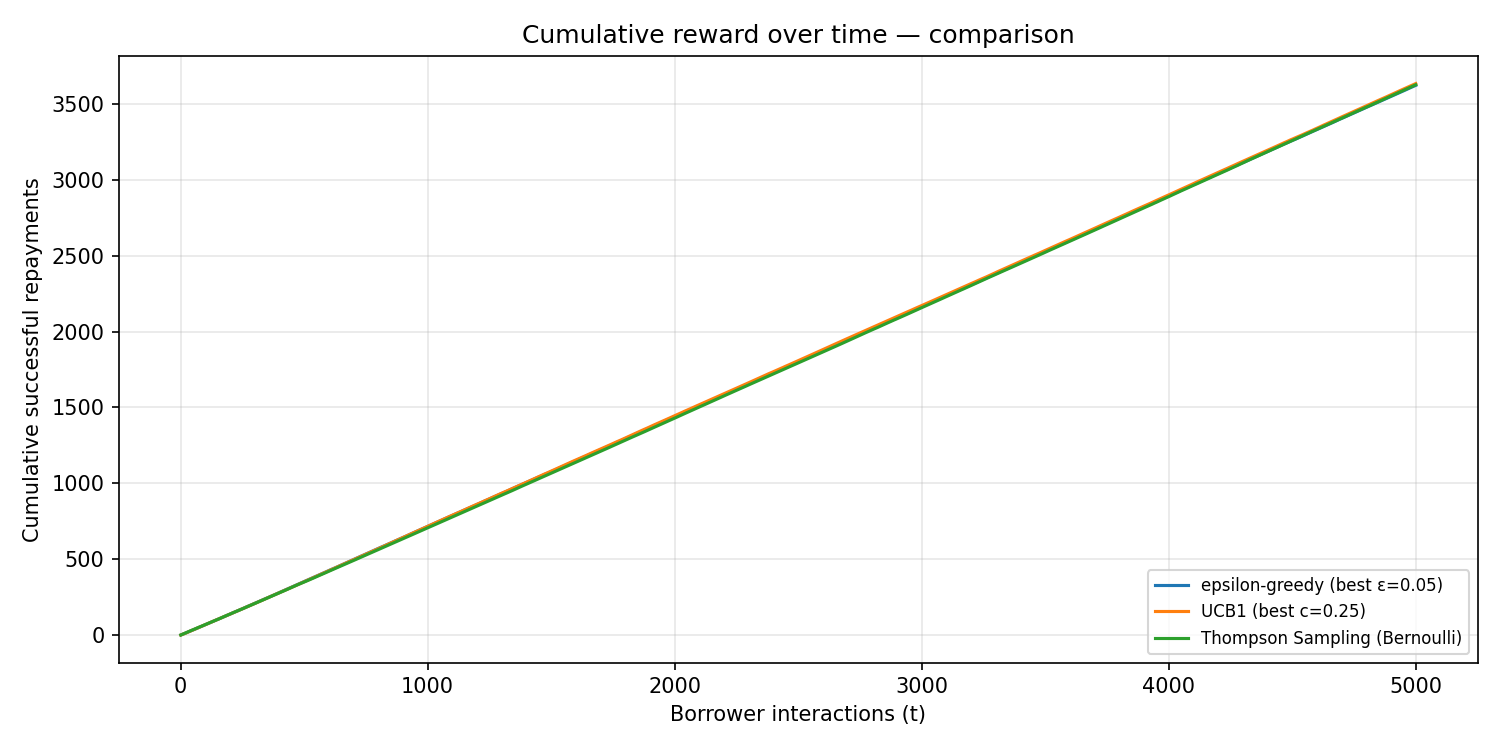
\includegraphics[width=0.95\linewidth]{comparison__cumulative_reward.png}
  \caption{Cumulative reward---final comparison.}
  \label{fig:comp-cum}
\end{figure}

\begin{figure}[htbp]
  \centering
  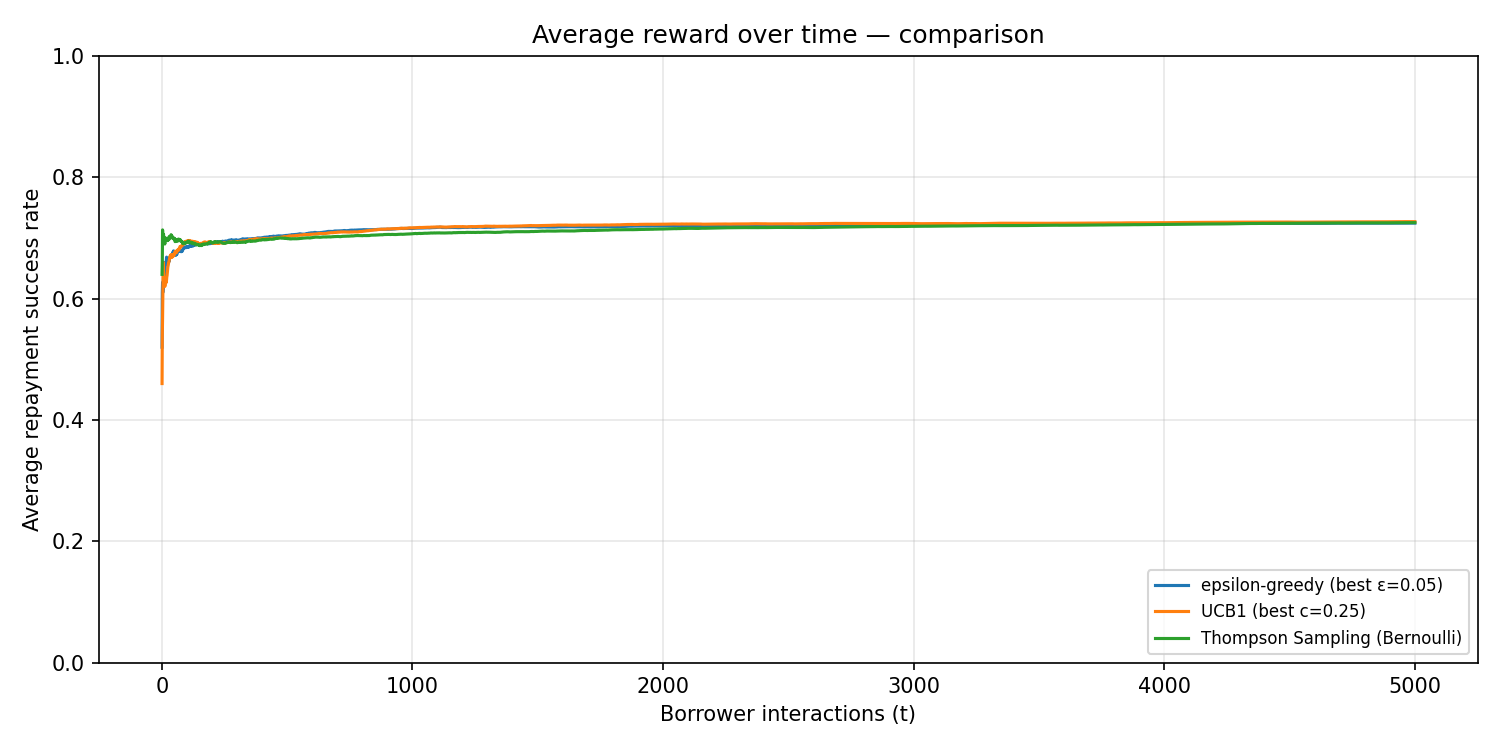
\includegraphics[width=0.95\linewidth]{comparison__average_reward.png}
  \caption{Average reward---final comparison.}
  \label{fig:comp-avg}
\end{figure}

\begin{figure}[htbp]
  \centering
  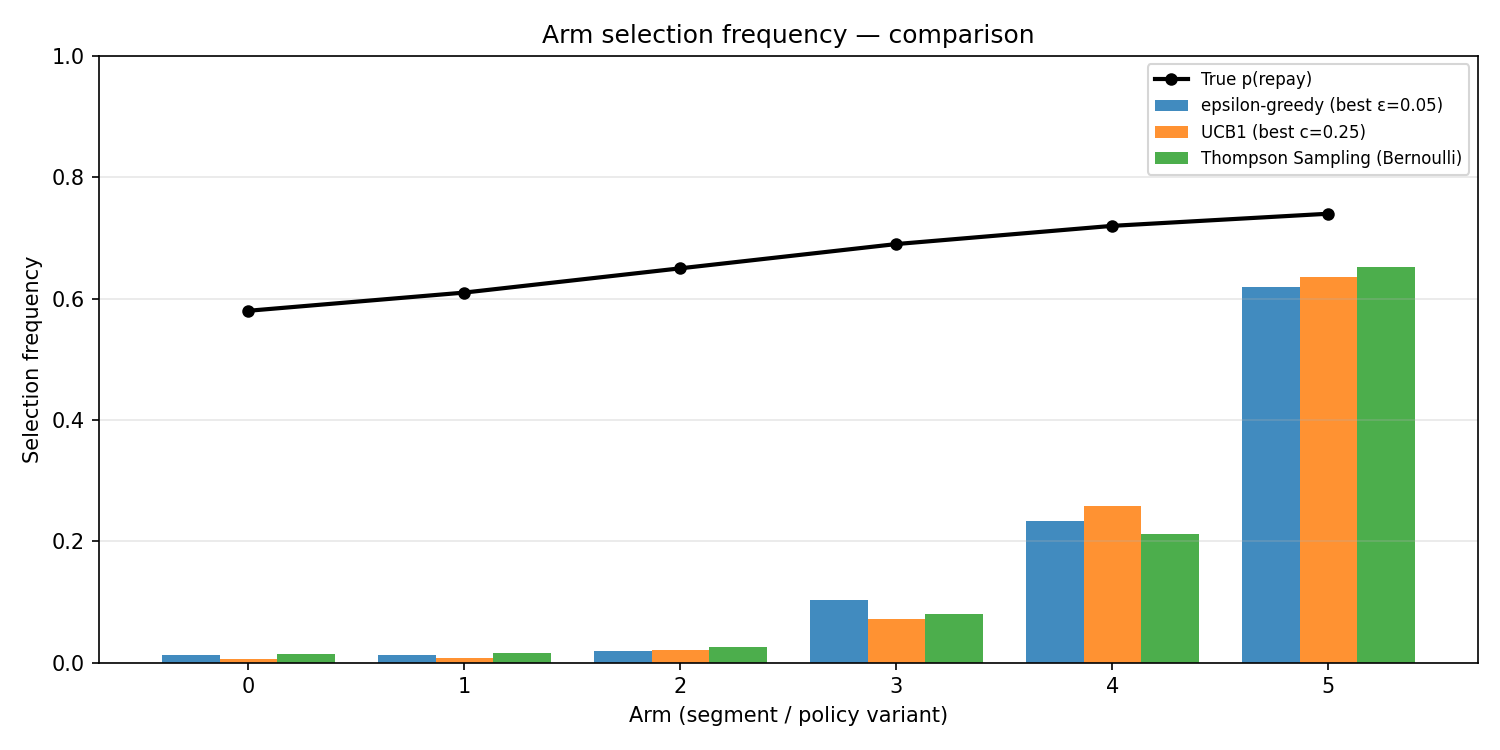
\includegraphics[width=0.85\linewidth]{comparison__arm_frequencies.png}
  \caption{Arm selection frequencies---final comparison. Black overlay: true $p_a$.}
  \label{fig:comp-freq}
\end{figure}

\section{Discussion and Analysis}

\subsection{Total reward earned}

Across $T{=}5000$ interactions, UCB1 with $c{=}0.25$ earned the most repayments ($3634.3$, average rate $0.7269$), outperforming the best $\varepsilon$-greedy setting by $11.6$ repayments and Thompson Sampling by $7.9$. All three algorithms improved cumulative reward over time (Figures~\ref{fig:eps-cum}--\ref{fig:comp-cum}), approaching but not reaching the oracle rate $0.74$ because exploration allocates some pulls to suboptimal segments.

\subsection{Exploration efficiency}

Regret quantifies wasted repayments relative to always selecting arm~5. UCB ($c{=}0.25$) achieved the lowest regret among final methods ($65.7$), versus $77.3$ for $\varepsilon$-greedy and $73.6$ for Thompson Sampling. Within the UCB sweep, increasing $c$ from $0.25$ to $2.00$ more than quadrupled regret ($65.7 \rightarrow 271.0$), showing that unstructured optimism can be as costly as excessive random exploration in $\varepsilon$-greedy ($\varepsilon{=}0.20$, regret $113.0$). UCB and Thompson Sampling explore \emph{where uncertainty is high}, whereas $\varepsilon$-greedy explores uniformly at rate $\varepsilon$.

\subsection{Exploitation effectiveness}

Tail best-arm rate measures how often the algorithm selects the true best segment once learning has progressed. Thompson Sampling leads ($0.840$), followed by UCB ($0.718$) and $\varepsilon$-greedy ($0.708$). The arm-frequency plots (Figures~\ref{fig:eps-freq}, \ref{fig:ucb-freq}, \ref{fig:comp-freq}) show increasing concentration on arm~5 for well-tuned settings; overtuned UCB ($c{=}2.00$, tail rate $0.300$) fails to exploit arm~5 consistently. $\varepsilon$-greedy continues random exploration even after convergence, capping exploitation relative to Thompson Sampling.

\subsection{Convergence speed}

Thompson Sampling reached $95\%$ of $p^\ast$ fastest ($t^\ast{=}6$), then UCB ($16$), then $\varepsilon$-greedy ($96$). Average-reward curves (Figures~\ref{fig:comp-avg} and sweep plots) rise steeply for Thompson Sampling and UCB early in the horizon. $\varepsilon{=}0.01$ was particularly slow ($t^\ast{=}268$) because it rarely probes alternative segments. Moderate $\varepsilon{=}0.05$ balanced speed and final performance within the epsilon sweep.

\subsection{Identifying the most creditworthy repeat borrowers}

All three final methods recovered the correct mean learned ranking ($5 > 4 > 3 > 2 > 1 > 0$), matching the true repayment ordering. Thompson Sampling's posterior means provide interpretable segment-level repayment beliefs. High tail best-arm rates and alignment of selection frequency with true $p_a$ in Figure~\ref{fig:comp-freq} indicate successful identification of the most creditworthy repeat-borrower segment.

\subsection{Suitability for adaptive credit scoring}

\begin{itemize}
  \item \textbf{$\varepsilon$-greedy} is a simple baseline for adaptive reapplication scoring but requires tuning $\varepsilon$. Our results show a $47$-repayment gap between the best and worst $\varepsilon$ in the sweep.
  \item \textbf{UCB1} is well suited when the system must learn systematically from limited segment data: best total reward and low regret with $c{=}0.25$, with deterministic decisions given history.
  \item \textbf{Thompson Sampling} is attractive when the lender wants calibrated uncertainty (Beta posteriors per segment), fast early learning ($t^\ast{=}6$), and strong late focus on the best segment (tail rate $0.84$), at a small cost in total reward versus UCB in this simulation.
\end{itemize}

Overall, exploration--exploitation bandits support repeat-borrower credit scoring by continuously updating segment creditworthiness from repayment outcomes. For this synthetic scenario, \textbf{UCB1} maximized repayments, while \textbf{Thompson Sampling} offered the fastest convergence and strongest identification of the best arm in the final phase.

\section{Implementation}

Source code: \texttt{bandits.py} (algorithms), \texttt{run\_experiments.py} (experiments and plots), \texttt{svg\_plots.py} (visualization). Run this command to get results:
\begin{verbatim}
python run_experiments.py --steps 5000 --sims 50 --seed 7 --outdir outputs
\end{verbatim}

\section*{References}
\addcontentsline{toc}{section}{References}
\begin{itemize}[noitemsep]
  \item Auer, Cesa-Bianchi, and Fischer (2002). Finite-time Analysis of the Multiarmed Bandit Problem.
  \item Thompson (1933). On the Likelihood that One Unknown Probability Exceeds Another.
  \item Sutton and Barto (2018). \emph{Reinforcement Learning: An Introduction} (bandits chapter).
\end{itemize}

\end{document}
